
\documentclass[14pt]{extarticle}
\usepackage{fontspec}
\usepackage{polyglossia} % use instead of babel
\usepackage{pgfplots}
\usepackage{float}
\usepackage{amsmath}
\usepackage{amsfonts}
\setdefaultlanguage{hebrew}
\setotherlanguage{english}
\newfontfamily\hebrewfont[Script=Hebrew]{Arial}

% TODO: figure out if better to keep this or not, for word document pdf output similarity
\usepackage[margin=1in]{geometry}

% might be useful to ensure similarity to word document pdf output
% \usepackage{setspace}
% \singlespacing

% Reset equation counter at the start of each section
\usepackage{chngcntr}
\usepackage{etoolbox}
\counterwithin*{equation}{section}
\preto{\section}{\setcounter{equation}{0}}

\begin{document}

\begin{center}
    {\LARGE \textbf{ממ"ן 16}}\\
    {\textbf{גלים במיתר}}
\end{center}

\begin{itemize}
    \item מגישים: תומר רוזנפלד, שי רואימי
    \item תאריך ביצוע הניסוי: 2 לספטמבר 2025
    \item מדריך הניסוי: ד"ר סילביו ריינהורן
\end{itemize}
\newpage
\section*{ניסוי 1 - כוחות בשדה מגנטי}
\subsection*{מטרת הניסוי}
מציאת עוצמת השדה המגנטי שמייצר מגנט, באמצעות מדידת הכוח המגנטי הפועל על תיל נושא זרם המונח בשדה.
\subsection*{רקע תיאורטי}
כאשר מוליך נושא זרם חשמלי נמצא בשדה מגנטי פועל עליו כוח מגנטי (כוח לורנץ)
הכוח נובע מאינטראקציה בין השדה המגנטי לבין המטענים הנעים בתיל.

גודלו של הכוח נתון ע"י חוק אמפר:
\begin{equation}
    F = I \cdot L \cdot B \cdot \sin(\theta)
\end{equation}

כאשר:
\begin{itemize}
    \item $F$ - גודל הכוח המגנטי (ניוטון)
    \item $I$ - עוצמת הזרם בתיל (אמפר)
    \item $L$ - אורך התיל בשדה המגנטי (מטר)
    \item $B$ - עוצמת השדה המגנטי (טסלה)
    \item $\theta$ - הזווית בין התיל לשדה המגנטי
\end{itemize}

את כיוון הכוח אפשר לקבוע באמצעות כלל יד שמאל.

\subsection*{מערכת המדידה ומהלך הניסוי}
בניסוי זה הנחנו מגנט קבוע על מאזניים דיגיטלים ואיפסנו את המשקל.

לאחר מכן חברנו לוחיות ועליהן תילים באורכים שונים לאמפר-מטר וספק זרם ישר. בעזרת זרוע אופקית מתקפלת מיקמנו את הלוחיות השונות בחלל שבין הקטבים של המגנט, כך שהתילים יהיו ניצבים לשדה המגנטי.

עבור זרם של 3.5 אמפר מדדנו את השינוי בקריאת המאזניים עבור אורכי תיל שונים.

מקריאת המאזניים הסקנו את הכוח המגנטי הפועל על התיל, ובאמצעות נוסחא (1) מצאנו את עוצמת השדה המגנטי.

לאחר מכן חיברנו למערכת תיל באורך 0.08 מטר ומדדנו את הכוח המגנטי שוב, עבור זרמים שונים, ושוב בעזרת נוסחא (1) מצאנו את עוצמת השדה המגנטי.

\subsection*{תוצאות וניתוח}

נשאלנו איזה חלק של התיל המודפס יפעיל כוח, ע"פ חוק אמפר רק החלק של התיל שכיוונו אנך לכיוון השדה המגנטי מפעיל כוח, ולכן רק חלקו התחתון של התיל נמדד.

תחילה מדדנו את קריאת המאזניים והכוח המגנטי עבור זרם של $3.5 [A]$ בשני הכיוונים

\begin{table}[H]
    \centering
    \renewcommand{\arraystretch}{1.5} % Increase row height
    \begin{tabular}{|p{2cm}|p{2.5cm}|p{2.5cm}|p{2.7cm}|p{2.7cm}|}
        \hline
        \textbf{אורך התיל} $[m]$ & \textbf{קריאת המאזניים} $[Kg]$ & \textbf{קריאת המאזניים בזרם הפוך} $[Kg]$ & \textbf{כוח מגנטי} $[N]$ & \textbf{כוח מגנטי בזרם הפוך} $[N]$ \\ \hline
        $1.2 \cdotp 10^{-2}$     & $-0.32 \cdotp 10^{-3}$         & $0.3 \cdotp 10^{-3}$                     & $-3.14 \cdotp 10^{-3}$   & $2.94 \cdotp 10^{-3}$              \\ \hline
        $2.2 \cdotp 10^{-2}$     & $-0.6 \cdotp 10^{-3}$          & $0.59 \cdotp 10^{-3}$                    & $-5.89 \cdotp 10^{-3}$   & $5.79 \cdotp 10^{-3}$              \\ \hline
        $3.2 \cdotp 10^{-2}$     & $-0.88 \cdotp 10^{-3}$         & $0.87 \cdotp 10^{-3}$                    & $-8.63 \cdotp 10^{-3}$   & $8.53 \cdotp 10^{-3}$              \\ \hline
        $4.2 \cdotp 10^{-2}$     & $-1.16 \cdotp 10^{-3}$         & $1.14 \cdotp 10^{-3}$                    & $-11.38 \cdotp 10^{-3}$  & $11.18 \cdotp 10^{-3}$             \\ \hline
        $6.4 \cdotp 10^{-2}$     & $-1.66 \cdotp 10^{-3}$         & $1.65 \cdotp 10^{-3}$                    & $-16.28 \cdotp 10^{-3}$  & $16.18 \cdotp 10^{-3}$             \\ \hline
        $8.4 \cdotp 10^{-2}$     & $-2.17 \cdotp 10^{-3}$         & $2.16 \cdotp 10^{-3}$                    & $-21.29 \cdotp 10^{-3}$  & $21.19 \cdotp 10^{-3}$             \\ \hline
    \end{tabular}
    \caption{מדידת הכוח המגנטי עבור זרם של 3.5 אמפר בשני הכיוונים}
    \label{tab:force_measurement}
\end{table}

נשרטט גרף של הכוח המגנטי F כתלות באורך התיל L, ונבצע התאמה ליניארית:

\begin{figure}[H]
    \centering
    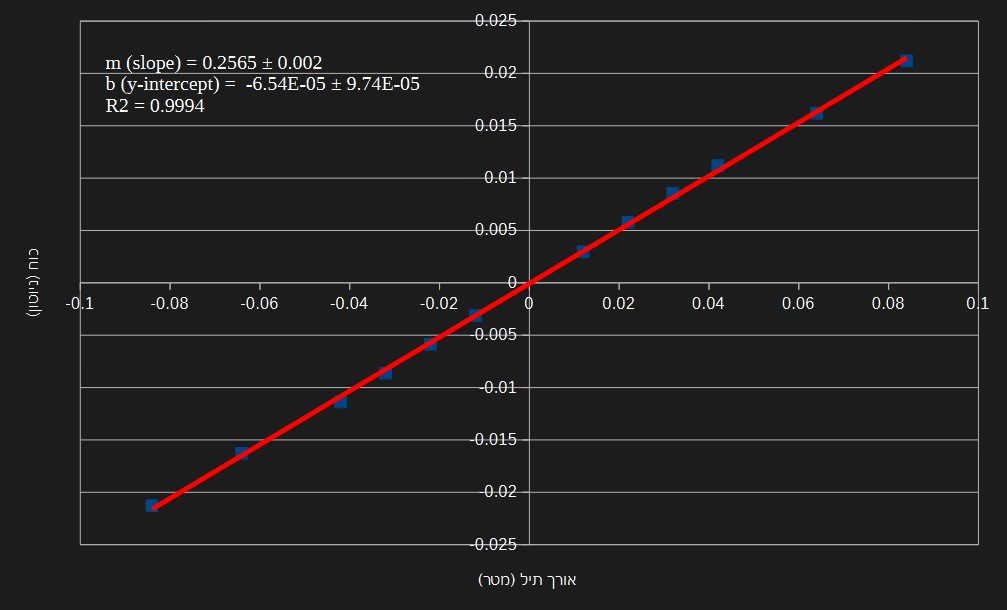
\includegraphics[width=0.7\textwidth]{magnetic_force_to_wire_length.jpg}
    \caption{קו מגמה עבור הכוח המגנטי כפונקציה של אורך התיל}
\end{figure}

שיפוע הגרף הוא $0.2565$ והשגיאה היא $0.002$.

כיוון  הכוח אנך לכיוון השדה המגנטי, ולכן בנוסחא (1) $\sin(\theta) = 1$.
כמו כן, בכל המדידות שנעשו הזרם היה $3.5 [A]$.
לפי נוסחא (1) נקבל:

\begin{center}
    \begin{equation*}
        \begin{aligned}
            F             & = I \cdot L \cdot B \cdot \sin(\theta) \\
            \sin(\theta)  & = 1                                    \\
            I             & = 3.5 [A]                              \\
            \Rightarrow F & = 3.5B \cdot L
        \end{aligned}
    \end{equation*}
\end{center}

כלומר שיפוע הגרף שווה ל $3.5B$, ומכאן שניתן למצוא את עוצמת השדה המגנטי:
\begin{equation*}
    0.2565 = 3.5B \Rightarrow B = \frac{0.2565}{3.5} = 0.0733 [T]
\end{equation*}

נחשב את השגיאה בשדה המגנטי מהשגיאה שניתנה בגרף מההתאמה הליניארית.

\begin{equation*}
    \Delta B  = \frac{m_{max} - m_{min}}{2 \cdot 3.5} = \frac{0.2585 - 0.2545}{2 \cdot 3.5} = \pm 0.007 [T]
\end{equation*}


נחשב כעת את שגיאת המדידה.

השגיאה במדידת האורך היא $\Delta L = 5 \cdot 10^{-4} [m]$.

שגיאת המדידה במאזניים היא:
\begin{equation*}
    \Delta m = 5 \cdot 10^{-6} [Kg]
\end{equation*}
ולכן השגיאה במדידת הכוח היא:
\begin{equation*}
    \Delta F = 5 \cdot 10^{-6} \cdot 9.81 \approx 4.9 \cdot 10^{-5} [N]
\end{equation*}

השגיאה באמפר-מטר במדידה של 3.5 אמפר היא $\Delta I = 0.05 [A]$.

נחשב את שגיאת המדידה:
\begin{equation*}
    \sigma = B \cdot (\frac{\Delta F}{F} + \frac{\Delta I}{I} + \frac{\Delta L}{L}) = 0.0733 \cdot (\frac{4.9 \cdot 10^{-5}}{2.94 \cdot 10^{-3}} + \frac{0.05}{3.5} + \frac{5 \cdot 10^{-4}}{1.2 \cdot 10^{-2}})
\end{equation*}
\begin{equation*}
    \sigma = 0.0733 \cdot (0.012 + 0.0143 + 0.042) = \pm 0.0683 [T]
\end{equation*}

לאחר מכן התבצע ניסוי דומה, בו אורך התיל היה קבוע ($0.08 [m]$) ועוצמת הזרם השתנתה. אלו התוצאות:

\begin{table}[H]
    \centering
    \renewcommand{\arraystretch}{1.5} % Increase row height
    \begin{tabular}{|c|c|c|}
        \hline
        \textbf{זרם} $[A]$ & \textbf{קריאת המאזניים} $[Kg]$ & \textbf{כוח  מגנטי} $[N]$ \\ \hline
        $1.07$             & $0.67 \cdotp 10^{-3}$          & $6.57 \cdotp 10^{-3}$     \\ \hline
        $1.61$             & $1.01 \cdotp 10^{-3}$          & $9.91 \cdotp 10^{-3}$     \\ \hline
        $2$                & $1.26 \cdotp 10^{-3}$          & $12.36 \cdotp 10^{-3}$    \\ \hline
        $2.53$             & $1.6 \cdotp 10^{-3}$           & $15.69 \cdotp 10^{-3}$    \\ \hline
        $3.11$             & $1.96 \cdotp 10^{-3}$          & $19.23 \cdotp 10^{-3}$    \\ \hline
        $3.53$             & $2.21 \cdotp 10^{-3}$          & $21.68 \cdotp 10^{-3}$    \\ \hline
        $3.96$             & $2.47 \cdotp 10^{-3}$          & $24.23 \cdotp 10^{-3}$    \\ \hline
        $4.45$             & $2.78 \cdotp 10^{-3}$          & $27.27 \cdotp 10^{-3}$    \\ \hline
    \end{tabular}
    \caption{מדידת הכוח המגנטי עבור אורך תיל קבוע של $0.08 [m]$ ועוצמת זרם משתנה}
    \label{tab:force_measurement}
\end{table}

את התוצאות נשרטט בגרף ונבצע התאמה ליניארית:
\begin{figure}[H]
    \centering
    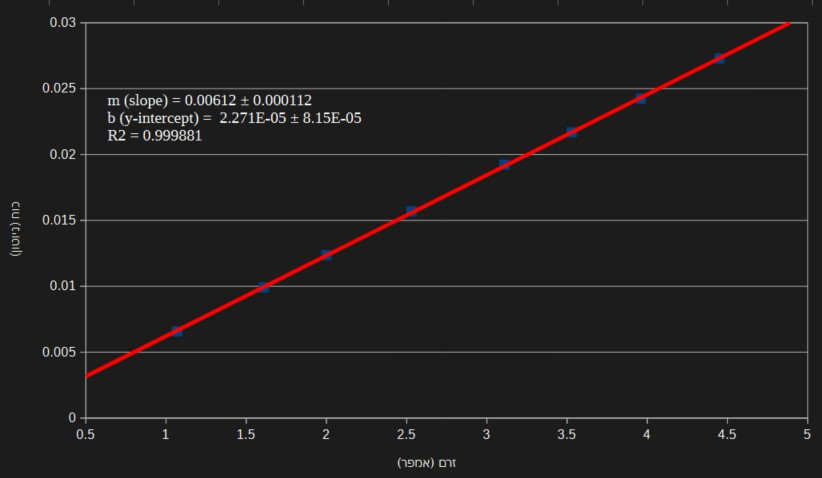
\includegraphics[width=0.7\textwidth]{magnetic_force_to_current.jpg}
    \caption{קו מגמה עבור הכוח המגנטי כפונקציה של עוצמת הזרם}
\end{figure}

נמצא שוב בעזרת נוסחא (1) את עוצמת השדה המגנטי:
\begin{center}
    \begin{equation*}
        \begin{aligned}
            F             & = I \cdot L \cdot B \cdot \sin(\theta) \\
            \sin(\theta)  & = 1                                    \\
            L             & = 0.08 [m]                             \\
            \Rightarrow F & = 0.08B \cdot I
        \end{aligned}
    \end{equation*}
\end{center}

כלומר שיפוע הגרף שווה ל $0.08B$, ומכאן שניתן למצוא את עוצמת השדה המגנטי:
\begin{equation*}
    0.00612 = 0.08B \Rightarrow B = \frac{0.00612}{0.08} = 0.0765 [T]
\end{equation*}

השגיאה שהתקבלה בשיפוע הגרף מההתאמה הליניארית היא $\pm 0.000112$. מכאן נמצא את השגיאה בשדה המגנטי:
\begin{equation*}
    \Delta B  = \frac{m_{max} - m_{min}}{2 \cdot 0.08} = \frac{0.006232 - 0.006008}{2 \cdot 0.08} = \pm 0.0014 [T]
\end{equation*}

בניסוי הקודם התקבלה התוצאה $B=0.0733 \pm 0.007 [T]$, ובניסוי זה $B=0.0765 \pm 0.0014 [T]$.
הסטייה היחסית בין שתי התוצאות היא:
\begin{equation*}
    \frac{|0.0765 - 0.0733|}{\frac{0.0765 + 0.0733}{2}} \approx 4.27 \%
\end{equation*}

\subsection*{דיון ומסקנות}
במדידות שבוצעו התקבל ערך לשדה המגנטי בסדר גודל של עשיריות טסלה, ערך סביר עבור מגנט קבוע, אך ללא ערך מדעי ידוע להשוואה – ולכן אין באפשרותנו לקבוע “נכונות מוחלטת” אלא רק עקביות עם התאוריה.

אכן נמצא קשר לינארי ברור בין הכוח לאורך התיל, וההתאמה הגרפית הצביעה על שגיאה סטטיסטית קטנה, מה שמעיד שהתיאוריה $F=ILB$ תאמה היטב לנתונים.


עם זאת, חישוב שגיאת המדידה על בסיס מגבלות המכשירים (רזולוציית מאזניים ודיוק אמפרמטר) נתן שגיאה גדולה בערך פי 10 מהשגיאה מהגרף. מכאן ניתן להסיק כי אמנם המודל הפיזיקלי מאושר היטב, אך הדיוק הכמותי של התוצאה מוגבל על־ידי איכות המכשור ולא על־ידי פיזור הנתונים.

\section*{ניסוי 2 - חישוב עוצמת השדה המגנטי של כדור הארץ}
\subsection*{מטרת הניסוי}
מדידת עוצמת השדה המגנטי של כדור הארץ באמצעות מדידת זווית הסטייה במצפן הנוצרת כתוצאה משדה מגנטי אנך לו.

\subsection*{רקע תיאורטי}
בניסוי זה נעזר  במכשיר הנקרא גלוונומטר טנגנטי על מנת למדוד את הרכיב האופקי של השדה המגנטי של כדור הארץ.

השדה המגנטי הנוצר על תיל בו זורם  ברם הוא:
\begin{equation}
    B = \frac{\mu_0 n}{2R} I
\end{equation}
כאשר:
\begin{itemize}
    \item $B$ - עוצמת השדה המגנטי (טסלה)
    \item $\mu_0$ - קבוע הפרמאביליות של הריק ($4\pi \cdot 10^{-7} [T \cdot m/A]$)
    \item $n$ - מספר הסלילים
    \item $R$ - רדיוס הסליל (מטר)
    \item $I$ - עוצמת הזרם בתיל (אמפר)
\end{itemize}

מצורפת דיאגרמה המציגה את השדה המגנטי של כדור הארץ ואת השדה המגנטי הנוצר על ידי הסליל:
\begin{figure}[H]
    \centering
    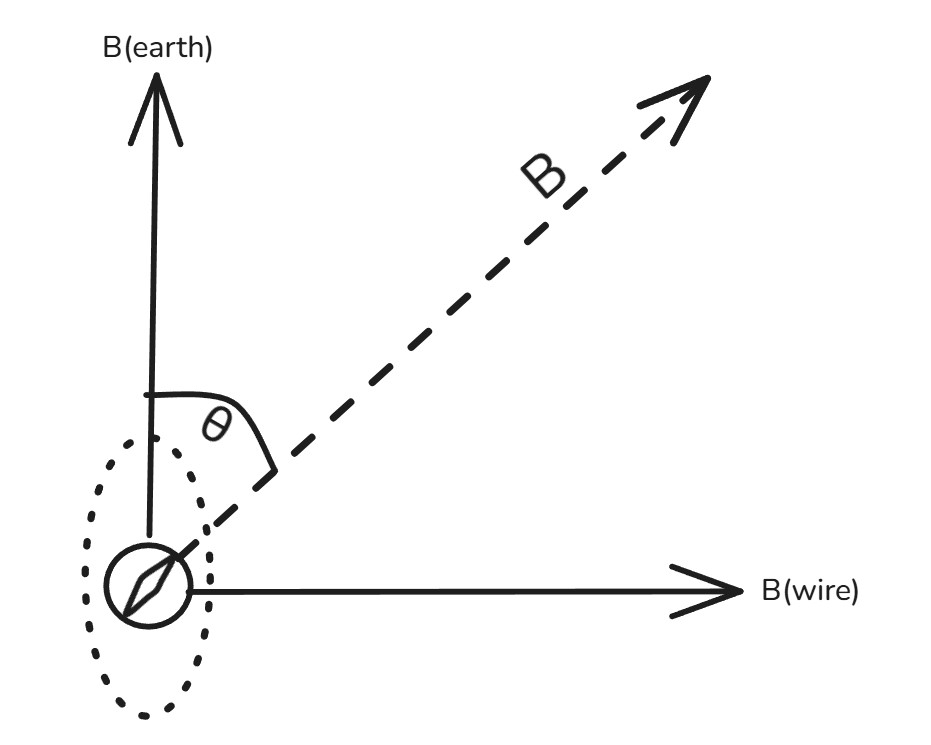
\includegraphics[width=0.5\textwidth]{magnetic_fields_diagram.jpg}
    \caption{דיאגרמה של השדה המגנטי של כדור הארץ ושל השדה המגנטי הנוצר על ידי הסליל}
\end{figure}

הזווית $\theta$ היא הזווית הסטייה של מחט המצפן מכיוונו המקורי של השדה המגנטי של כדור הארץ כתוצאה מהשדה הנוצר מהזרם בתיל.

נשים לב כי:
\begin{equation}
    \tan(\theta) = \frac{B_{wire}}{B_{earth}}
\end{equation}

ולכן:
\begin{equation}
    \tan(\theta) = \frac{\mu_0 n}{2R B_{earth}}I
\end{equation}

\subsection*{מערכת המדידה ומהלך הניסוי}
בניסוי זה חיברנו גלוונומטר טנגנטי לספר זרם ישר ואמפרמטר.

הרכבנו מעגל חשמלי, ראשית עם שלושה ליפופים ומדדנו את השינוי הנדרש בזרם לשינוי הזווית ב10 מעלות, החל מ20 מעלות עד 60 מעלות.

את הפעולה הזאת ביצענו לשני הכיוונים של הזרם, ולאחר מכן עם מספר גדול יותר של ליפופים (15).

בשני המקרים חישנו את $B_earth$ בעזרת היחס שבנוסחא (3) והשוו את התוצאות את לשנייה ולערך הידוע בספרות.

\subsection{תוצאות וניתוח}
ראשית יש לציין, רדיוס הגלוונומטר (נמדד בסרגל) הוא $R=0.1025 [m]$.

עבור שלושה ליפופים, הזרמים שהתקבלו לשינויים ב10 מעלות היו:

\begin{center}
    \begin{tabular}{|c|c|c|c|c|c|c|}
        \hline
        $\theta\ [\deg]$ & $0$ & $+20$  & $+30$  & $+40$  & $+50$  & $+60$  \\
        \hline
        $I [A]$          & $0$ & $0.56$ & $0.88$ & $1.27$ & $1.84$ & $2.65$ \\
        \hline
    \end{tabular}
\end{center}

\begin{center}
    \begin{tabular}{|c|c|c|c|c|c|c|}
        \hline
        $\theta\ [\deg]$ & $0$ & $-20$  & $-30$  & $-40$  & $-50$  & $-60$  \\
        \hline
        $I [A]$          & $0$ & $0.57$ & $0.75$ & $1.17$ & $1.76$ & $2.43$ \\
        \hline
    \end{tabular}
\end{center}

נשרטט גרף של  $tan(\theta)$ כפונקציה של הזרם $I$ ונבצע התאמה ליניארית:
\begin{figure}[H]
    \centering
    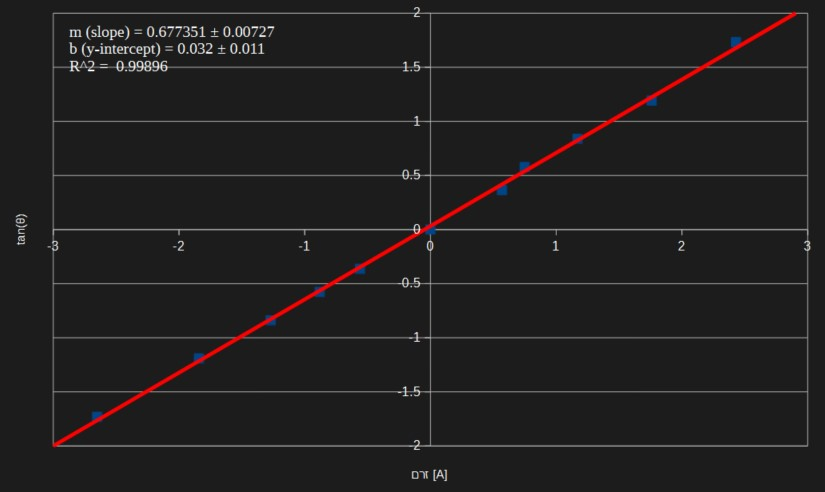
\includegraphics[width=0.7\textwidth]{tangent_angle_to_current_3_loops.jpg}
    \caption{קו מגמה עבור $\tan(\theta)$ כפונקציה של הזרם עבור 3 ליפופים}
\end{figure}

השיפוע מההתאמה הליניארית הוא 0.677351 והשגיאה מהגרף היא $±0.00727$.
נחשב את עוצמת השדה המגנטי של כדור הארץ בעזרת נוסחא (3):
\begin{center}
    \begin{equation*}
        \begin{aligned}
            \tan(\theta) & = \frac{\mu_0 n}{2R B_{earth}}I \Rightarrow B_{earth} = \frac{\mu_0 n}{2R \cdot \text{שיפוע}} \\
            \mu_0        & = 4\pi \cdot 10^{-7} [T \cdot m/A]                                                            \\
            n            & = 3                                                                                           \\
            R            & = 0.1025 [m]                                                                                  \\
            B_{earth}    & = \frac{4\pi \cdot 10^{-7} \cdot 3}{2 \cdot 0.1025 \cdot 0.677351} = 2.715 \cdot 10^{-5} [T]
        \end{aligned}
    \end{equation*}
\end{center}

לאחר מכן חזרנו על הניסוי כאשר בסליל 15 ליפופים:

\begin{center}
    \begin{tabular}{|c|c|c|c|c|c|c|}
        \hline
        $\theta\ [\deg]$ & $0$ & $+20$  & $+30$  & $+40$  & $+50$  & $+60$  \\
        \hline
        $I [A]$          & $0$ & $0.08$ & $0.14$ & $0.24$ & $0.32$ & $0.47$ \\
        \hline
    \end{tabular}
\end{center}

\begin{center}
    \begin{tabular}{|c|c|c|c|c|c|c|}
        \hline
        $\theta\ [\deg]$ & $0$ & $-20$  & $-30$  & $-40$  & $-50$  & $-60$  \\
        \hline
        $I [A]$          & $0$ & $0.09$ & $0.14$ & $0.21$ & $0.33$ & $0.47$ \\
        \hline
    \end{tabular}
\end{center}

נשרטט שוב גרף של  $tan(\theta)$ כפונקציה של הזרם $I$ ונבצע התאמה ליניארית:
\begin{figure}[H]
    \centering
    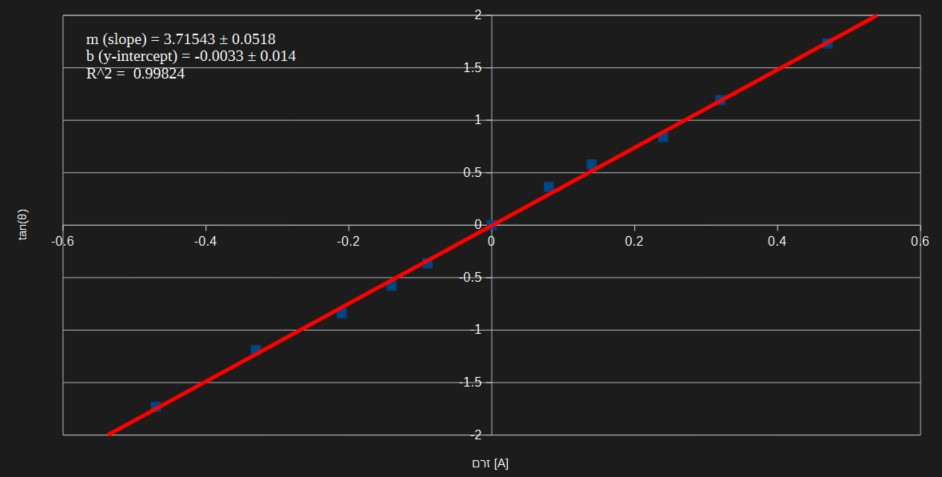
\includegraphics[width=0.7\textwidth]{tangent_angle_to_current_15_loops.jpg}
    \caption{קו מגמה עבור $\tan(\theta)$ כפונקציה של הזרם עבור 15 ליפופים}
\end{figure}

השיפוע מההתאמה הליניארית הוא 3.71543 והשגיאה מהגרף היא $±0.0518$.

נחשב את עוצמת השדה המגנטי של כדור הארץ בעזרת נוסחא (3):
\begin{center}
    \begin{equation*}
        \begin{aligned}
            \tan(\theta) & = \frac{\mu_0 n}{2R B_{earth}}I \Rightarrow B_{earth} = \frac{\mu_0 n}{2R \cdot \text{שיפוע}} \\
            \mu_0        & = 4\pi \cdot 10^{-7} [T \cdot m/A]                                                            \\
            n            & = 15                                                                                          \\
            R            & = 0.1025 [m]                                                                                  \\
            B_{earth}    & = \frac{4\pi \cdot 10^{-7} \cdot 15}{2 \cdot 0.1025 \cdot 3.71543} = 2.475 \cdot 10^{-5} [T]
        \end{aligned}
    \end{equation*}
\end{center}

הערך המומצע משתי המדידות הוא:
\begin{equation*}
    B_{earth} = \frac{2.715 + 2.475}{2} \cdot 10^{-5} = 2.595 \cdot 10^{-5} [T]
\end{equation*}

\subsection{דיון ומסקנות}

השגיאה היחסית בין הערך המומצע לערך הידוע היא:
\begin{equation*}
    \frac{|2.99 - 2.595|}{2.99} \approx 13.21 \%
\end{equation*}

סיבות לשגיאה יכולות להיות שגיאות מדידה, באמפר-מטר שגיאת המדידה  היא 0.05 אמפר, שגיאת מדידה  בסרגל במדידת רדיוס הגלוונמטר (0.0005 מטר)
ושגיאת מדידה בסטיית הזווית במצפן (חצי מעלה).

מעבר לכך, השגיאה   יכולה לנבוע גם כתוצאה מהפרעות סביבתיות (מתכות או מכשירים חשמליים בקרבת מקום).

\end{document}